\documentclass[a4paper,11pt,UTF8]{article}
\usepackage{ctex}
\usepackage{amsmath,amsthm,amssymb,amsfonts}
\usepackage{amsmath}
\usepackage[a4paper]{geometry}
\usepackage{graphicx}
\usepackage{microtype}
\usepackage{siunitx}
\usepackage{booktabs}
\usepackage[colorlinks=false, pdfborder={0 0 0}]{hyperref}
\usepackage{cleveref}
\usepackage{esint} 
\usepackage{graphicx}
\usepackage{ragged2e}
\usepackage{pifont}
\usepackage{extarrows}
\usepackage{mathptmx}
\usepackage{float}
\usepackage{caption}
\usepackage{multirow}
\usepackage{subfigure}
\usepackage{titlesec}
\captionsetup[figure]{name={图}}
%opening
\title{数字电子技术作业(五)}
\author{谢悦晋 \quad U202210333}
\date{Nov 6th, 2023 }
\begin{document}
\maketitle
\textbf{6.2.4} 试分析图题 6.2.4 所示电路,列出状态转换表,并画出状态转换图。当输入序列$A$为01011011111111101,其输出序列 $Z$ 是什么? 该电路可以检测 $A$ 的何种输入序列?
\begin{figure}[H]
	\centering
	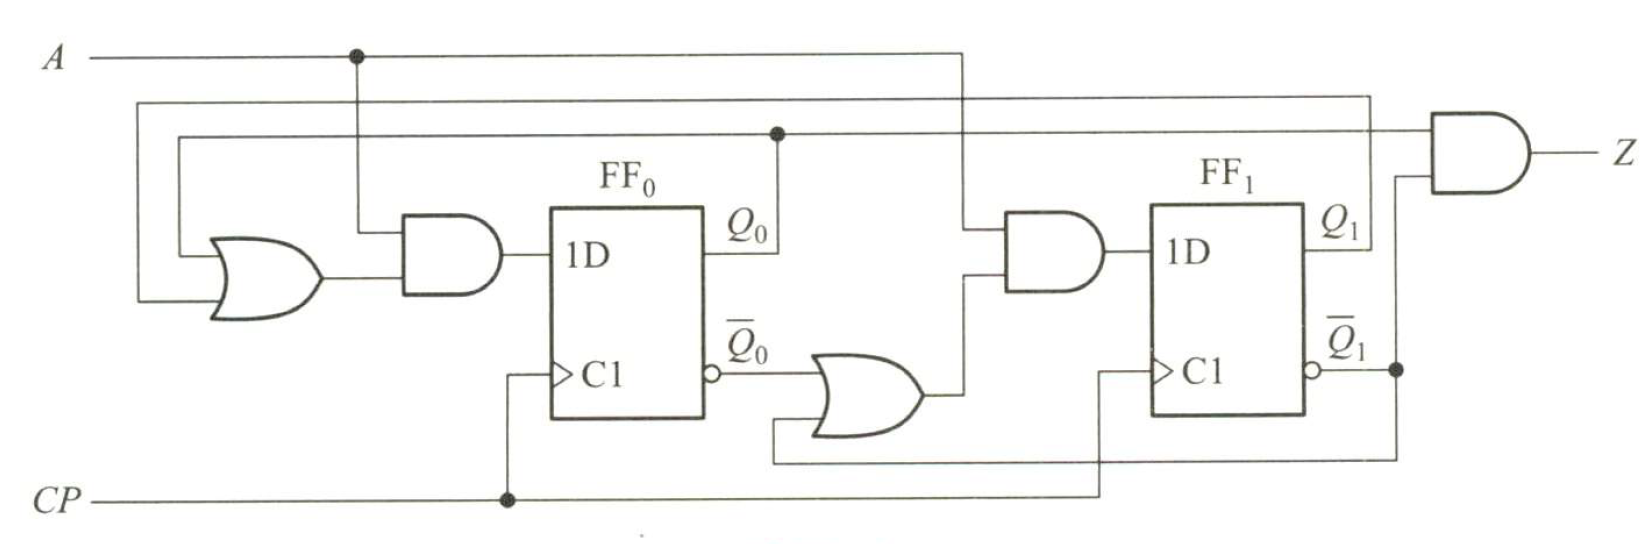
\includegraphics[width=0.9\textwidth]{6.2.4}
\end{figure}
\textbf{6.2.6} 试分析图题 6.2.6 所示同步时序电路,写出激励方程组、状态转换方程组和输出方程,列出状态转换表并画出状态转换图。
\begin{figure}[H]
	\centering
	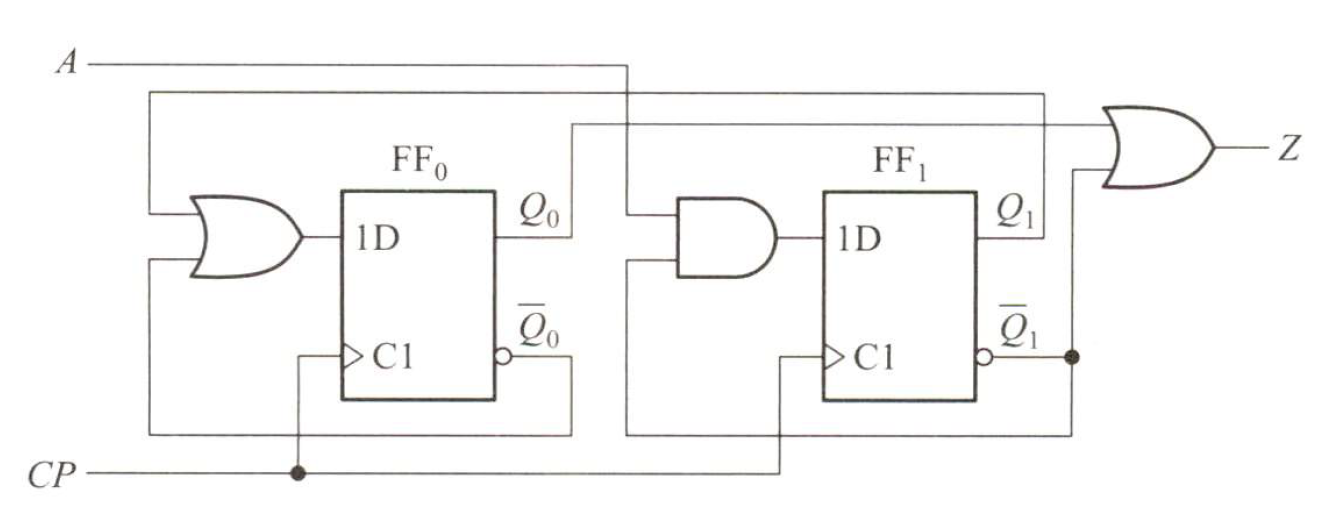
\includegraphics[width=0.9\textwidth]{6.2.6}
\end{figure}
\textbf{6.3.5} 试用下降沿触发的$JK$触发器和最少的门电路,实现图题 6.3.5 所示的$Z_{1}$和$Z_{2}$输出波形(要求写出Verilog程序)
\begin{figure}[H]
	\centering
	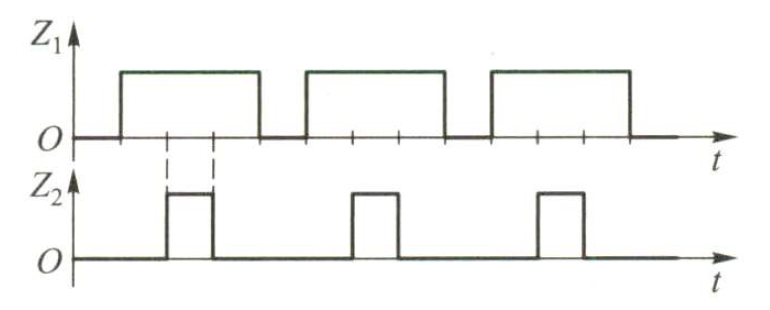
\includegraphics[width=0.7\textwidth]{6.3.5}
\end{figure}
\textbf{6.3.6} 试用上升沿触发的$D$触发器设计一个1101序列检测器(序列可重复),输入为串行编码序列,输出为检出信号(要求写出Verilog程序)

\end{document}